\documentclass[tikz,border=5mm]{standalone}
\usepackage{xcolor}

\definecolor{gameblue}{RGB}{0, 102, 204}

\begin{document}
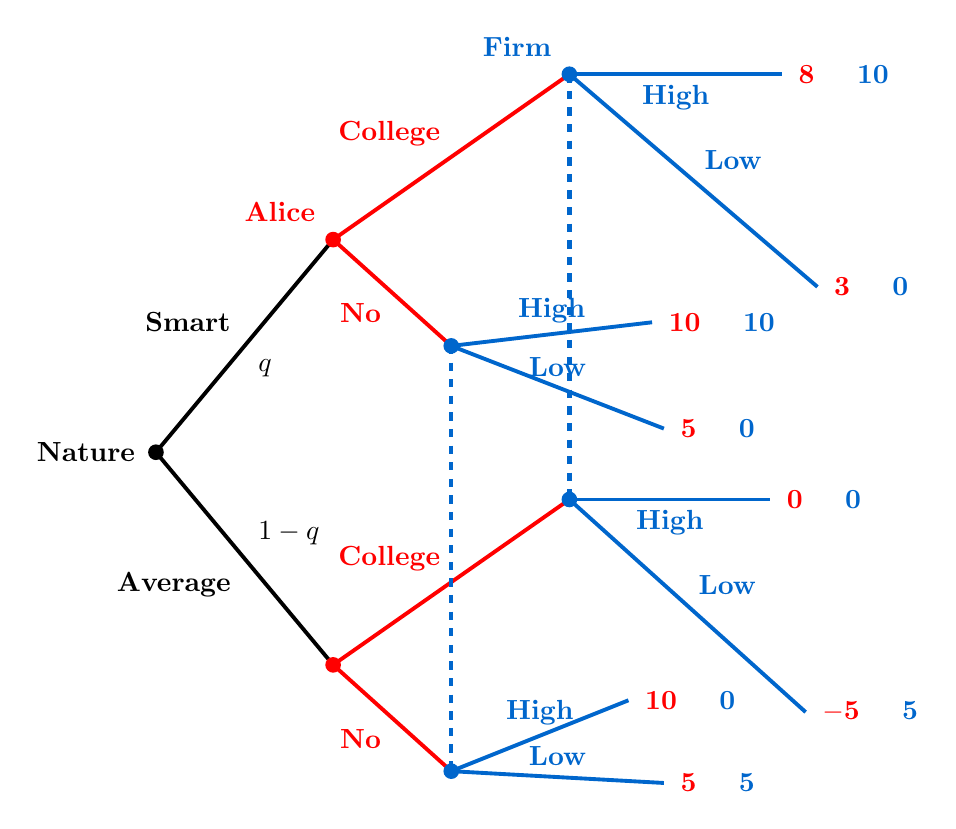
\begin{tikzpicture}[
    scale=1.5,
    font=\bfseries,
    dot/.style={circle, fill=#1, inner sep=2pt},
    dot/.default=black,
    line width=1.4pt
]

    % ==========================================
    % COORDINATES
    % ==========================================
    % Root (Nature)
    \coordinate (root) at (0, 0);

    % Alice's Nodes
    \coordinate (alice_top) at (1.5, 1.8);
    \coordinate (alice_bot) at (1.5, -1.8);

    % Firm's Nodes (College: x = 3.5, No: x = 2.5)
    \coordinate (firm_tc) at (3.5, 3.2);  % Top College
    \coordinate (firm_tn) at (2.5, 0.9);  % Top No
    \coordinate (firm_bc) at (3.5, -0.4); % Bottom College
    \coordinate (firm_bn) at (2.5, -2.7); % Bottom No

    % Payoff Endpoints - Top College
    \coordinate (l_tc_high) at (5.3, 3.2);
    \coordinate (l_tc_low)  at (5.6, 1.4);

    % Payoff Endpoints - Top No
    \coordinate (l_tn_high) at (4.2, 1.1);
    \coordinate (l_tn_low)  at (4.3, 0.2);

    % Payoff Endpoints - Bottom College
    \coordinate (l_bc_high) at (5.2, -0.4);
    \coordinate (l_bc_low)  at (5.5, -2.2);

    % Payoff Endpoints - Bottom No
    \coordinate (l_bn_high) at (4.0, -2.1);
    \coordinate (l_bn_low)  at (4.3, -2.8);


    % ==========================================
    % LEVEL 1: NATURE (Black)
    % ==========================================
    \draw[black] (root) -- (alice_top) 
        node[midway, above left=1pt] {Smart}
        node[midway, below right=1pt] {$q$};
        
    \draw[black] (root) -- (alice_bot) 
        node[midway, below left=1pt] {Average}
        node[midway, above right=1pt] {$1-q$};


    % ==========================================
    % LEVEL 2: ALICE (Red)
    % ==========================================
    % Top Alice
    \draw[red] (alice_top) -- (firm_tc) node[midway, above left] {College};
    \draw[red] (alice_top) -- (firm_tn) node[midway, below left] {No};

    % Bottom Alice
    \draw[red] (alice_bot) -- (firm_bc) node[midway, above left] {College};
    \draw[red] (alice_bot) -- (firm_bn) node[midway, below left] {No};


    % ==========================================
    % INFORMATION SETS (Firm - Blue Dashed)
    % ==========================================
    \draw[gameblue, dashed, line width=1.6pt] (firm_tc) -- (firm_bc);
    \draw[gameblue, dashed, line width=1.6pt] (firm_tn) -- (firm_bn);


    % ==========================================
    % LEVEL 3: FIRM (Blue)
    % ==========================================
    % Top College
    \draw[gameblue] (firm_tc) -- (l_tc_high) node[midway, below] {High};
    \draw[gameblue] (firm_tc) -- (l_tc_low)  node[midway, above right] {Low};

    % Top No
    \draw[gameblue] (firm_tn) -- (l_tn_high) node[midway, above] {High};
    \draw[gameblue] (firm_tn) -- (l_tn_low)  node[midway, above] {Low};

    % Bottom College
    \draw[gameblue] (firm_bc) -- (l_bc_high) node[midway, below] {High};
    \draw[gameblue] (firm_bc) -- (l_bc_low)  node[midway, above right] {Low};

    % Bottom No
    \draw[gameblue] (firm_bn) -- (l_bn_high) node[midway, above] {High};
    \draw[gameblue] (firm_bn) -- (l_bn_low)  node[midway, above] {Low};


    % ==========================================
    % NODES & PLAYER LABELS
    % ==========================================
    \node[dot=black, label=left:Nature] at (root) {};
    
    \node[dot=red, label={[red]above left:Alice}] at (alice_top) {};
    \node[dot=red] at (alice_bot) {};
    
    \node[dot=gameblue, label={[gameblue]above left:Firm}] at (firm_tc) {};
    \node[dot=gameblue] at (firm_tn) {};
    \node[dot=gameblue] at (firm_bc) {};
    \node[dot=gameblue] at (firm_bn) {};


    % ==========================================
    % PAYOFFS (Alice: Red, Firm: Blue)
    % ==========================================
    % Top College
    \node[right=2pt] at (l_tc_high) {\textcolor{red}{8} \quad \textcolor{gameblue}{10}};
    \node[right=2pt] at (l_tc_low)  {\textcolor{red}{3} \quad \textcolor{gameblue}{0}};

    % Top No
    \node[right=2pt] at (l_tn_high) {\textcolor{red}{10} \quad \textcolor{gameblue}{10}};
    \node[right=2pt] at (l_tn_low)  {\textcolor{red}{5} \quad \textcolor{gameblue}{0}};

    % Bottom College
    \node[right=2pt] at (l_bc_high) {\textcolor{red}{0} \quad \textcolor{gameblue}{0}};
    \node[right=2pt] at (l_bc_low)  {\textcolor{red}{$-$5} \quad \textcolor{gameblue}{5}};

    % Bottom No
    \node[right=2pt] at (l_bn_high) {\textcolor{red}{10} \quad \textcolor{gameblue}{0}};
    \node[right=2pt] at (l_bn_low)  {\textcolor{red}{5} \quad \textcolor{gameblue}{5}};

\end{tikzpicture}
\end{document}
